\begin{lpu}

Maschinelles Lernen lebt von den Daten – ohne Daten keine Erkenntnis. Damit Sie sinnvolle Modelle entwickeln k\"onnen, m\"ussen Sie Ihre Daten kennen, analysieren und korrekt aufbereiten. Das beginnt damit, die unterschiedlichen Datentypen zu verstehen, die im maschinellen Lernen auftreten. Nur so k\"onnen Sie entscheiden, welcher Algorithmus sich f\"ur Ihre Aufgabenstellung eignet.

\begin{aufgabe}{1}
Betrachten Sie die folgende Tabelle mit Informationen zu fiktiven Personen: \vspace{0.5em}

\begin{center}
\begin{tabular}{|l|l|l|l|l|}
\hline
\textbf{Name} & \textbf{Alter} & \textbf{Geschlecht} & \textbf{Gewicht (in kg)} & \textbf{Region} \\
\hline
Anna   & 22    & weiblich  & 55   & Nordwest \\
Luca   & 35    & m\"annlich & 82   & S\"udost \\
Fatima & 41    & weiblich  & 63  & Zentrum \\
\hline
\end{tabular}
\end{center}

Sehen Sie Unterschiede in der Art dieser Daten? Versuchen Sie in Worte zu fassen, worin sich die einzelnen Spalten unterscheiden.

\textbf{Hinweis:} Stellen Sie sich die Frage: \textit{Welche dieser Angaben kann ich sinnvoll miteinander verrechnen, zum Beispiel, um den Durchschnitt zu bestimmen?}
\end{aufgabe}

Es gibt ganz unterschiedliche Arten, Daten einzuordnen und zu analysieren. Doch für diese Unterrichtseinheit ist die nachfolgende Unterscheidung zielführend, weil sie uns später erlaubt, die richtigen Methoden auszusuchen.

\begin{theorie}
Im maschinellen Lernen unterscheidet man zwei Arten von Daten:
\begin{itemize}
  \item \textbf{numerische Daten} (\emph{numerical data}): messbare Werte wie Alter, Temperatur oder Einkommen. Diese kann man verrechnen.
  \item \textbf{kategorische Daten} (\emph{categorical data}): beschreibende Werte wie Farbe, Geschlecht oder Region. Diese kann man nicht sinnvoll verrechnen.
\end{itemize}
\end{theorie}

\begin{aufgabe}{2}
Ordnen Sie folgende Merkmale einer Person den zwei Datentypen zu: \emph{Alter, Geschlecht, Nationalit\"at, Gewicht, Wohnregion, Schulabschluss}. Begr\"unden Sie Ihre Entscheidungen.
\end{aufgabe}

Im Beispiel oben ist die Zuordnung weitgehend eindeutig: Man kann sich zwar überlegen, ob man bei Schulabschluss eine Note ausgibt oder auflistet, ob jemand eine EFZ, eine Matur oder einen anderen Abschluss gemacht hat. Im ersten Fall hätten wir es dann mit \textit{numerischen} Daten zu tun, und im zweiten Fall mit \textit{kategorischen}. Doch aufgepasst! Was, wenn wir alle möglichen Abschlüsse auflisten, und nur die \textbf{Nr.} verwenden, um anzugeben, welchen Abschluss jemand erreicht hat?

\begin{table}
\begin{center}
\begin{tabular}{|c|l|}
\hline
\textbf{Nr.} & \textbf{Abschluss} \\
\hline
1 & obligatorische Schule abgeschlossen \\
2 & Berufslehre mit EFZ \\
3 & Berufsmaturität \\
4 & Fachmittelschule (FMS) \\
5 & Gymnasiale Maturität \\
6 & Höhere Fachschule (HF) \\
7 & Fachhochschule (FH) Bachelor \\
8 & Universität / ETH Bachelor \\
9 & Fachhochschule (FH) Master \\
10 & Universität / ETH Master \\
11 & Doktorat (Dr./PhD) \\
\hline
\end{tabular}
\caption{Typische schulische und tertiäre Abschlüsse in der Schweiz, nummeriert.}
\label{tab:abschluesse}
\end{center}
\end{table}

Aufgepasst also vor \textbf{falschen Freunden}! In diesem Fall sind 5, 7 und 8 (zum Beispiel) zwar Zahlen, aber stellen trotzdem \textit{kategorische} Daten dar. Wir können zwar theoretisch diese Zahlen verrechnen, doch bedeuten die numerischen Werte nichts. Welchem Abschluss würde eine 3.5 entsprechen?

\begin{theorie}
Viele Algorithmen im ML k\"onnen nur mit Zahlen arbeiten. Deshalb m\"ussen kategorische Daten oft in Zahlen umgewandelt werden. Die Daten bleiben kategorisch, wobei jeder Kategorie eine Zahl zugeordnet wird.
\end{theorie}

Auch numerische Daten m\"ussen oft vorbereitet werden: Manche ML-Algorithmen reagieren empfindlich darauf, wenn sich numerische Werte nicht zwischen $[0,1]$ bewegen. Das nachfolgende Beispiel veranschaulicht dies:

\begin{aufgabe}{3}
Sie haben einen Datensatz (Person X) mit den Werten: \texttt{Alter = 28}, \texttt{Einkommen = 78000 CHF}. Welche der folgenden Personen ist \textit{ähnlicher}? Begründen Sie Ihre Wahl:
\begin{itemize}
  \item Person A: Alter = 26, Einkommen = 50\,000
  \item Person B: Alter = 40, Einkommen = 79\,000
\end{itemize}
Wie würden Sie argumentieren, wenn Sie erfahren würden, dass die \textit{andere} Person, als die, für die Sie sich ursprünglich entschieden haben, ähnlicher wäre?
\end{aufgabe}

Die Intuitionen können hier auseinander gehen, und für einen Computer reichen solche sowieso nicht aus: Wir müssen den \textit{Abstand} von X zu A und zu B mathematisch sauber definieren, damit wir die Frage beantworten können.

Ein naiver Ansatz wäre, diesen Abstand zwischen den Personen so zu berechnen, dass wir also die Differenz in den einzelnen Merkmalen aufsummieren.

\textbf{Abstand zu Person A:} $|28 - 26| + |78\,000 - 50\,000| = 2 + 28\,000 = 28\,002$ \\
\textbf{Abstand zu Person B:} $|28 - 40| + |78\,000 - 79\,000| = 12 + 1000 = 1012$

Dieser Vergleich zeigt ein Problem: Das Einkommen überwiegt aufgrund seines viel grösseren Zahlenbereichs deutlich. In dieser Rechenart müsste Person B 27\,003 Jahre alt sein, bevor sie X ähnlicher als A wäre. Völlig sinnlos, denn wer ein solches Alter erreicht, hat ungeachtet der Einkommensverhältnisse mit niemandem überhaupt eine Ähnlichkeit!

Unser Algorithmus „sieht“ also fast nur den Unterschied im Einkommen; einfach deshalb, weil sich das Einkommen in viel grösseren Dimensionen bewegt als das Alter. In der Schweiz bewegt sich der Lohn für 80\% der Einwohner zwischen 36\,000 und 120\,000 Franken; die älteste Schweizerin ist fast 113 Jahre alt geworden.

Genau hier kommt das sogenannte \emph{Skalieren} ins Spiel. Um  Merkmale vergleichbar zu machen, die auf unterschiedlichen Grössenordnungen gemessen werden, werden sie auf denselben Wertebereich gebracht – meistens auf ein Intervall zwischen 0 und 1. 

\begin{theorie}
    Um einen Wertebereich zu skalieren, geht man wie folgt vor: Man bestimmt für jedes Merkmal den kleinsten und grössten Wert im Datensatz, und rechnet dann:
    \[
\text{Skalierter Wert} = \frac{\text{aktueller Wert} - \text{Minimum}}{\text{Maximum} - \text{Minimum}}
\]
\end{theorie}

\textbf{Skalierung visuell erklärt:}

\begin{center}
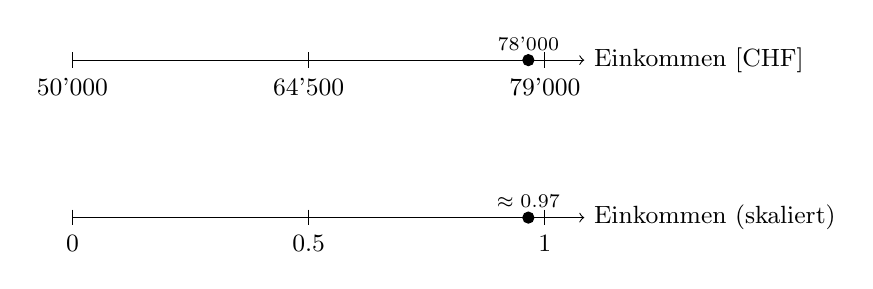
\begin{tikzpicture}
  % Achse Einkommen (original)
  \draw[->] (0,0) -- (6.5,0) node[right] {\small Einkommen [CHF]};
  \foreach \x/\v in {0/50'000, 3/64'500, 6/79'000} {
    \draw (\x,0.1) -- (\x,-0.1) node[below] {\small \v};
  }
  \draw[fill=black] (5.79,0) circle (2pt) node[above] {\scriptsize 78'000};

  % Achse Einkommen (skaliert)
  \draw[->] (0,-2) -- (6.5,-2) node[right] {\small Einkommen (skaliert)};
  \foreach \x/\v in {0/0, 3/0.5, 6/1} {
    \draw (\x,-1.9) -- (\x,-2.1) node[below] {\small \v};
  }
  \draw[fill=black] (5.79,-2) circle (2pt) node[above] {\scriptsize $\approx 0.97$};
\end{tikzpicture}
\end{center}



Wie die Abbildung zeigt, wird ein Wert wie 78\,000 CHF durch die Skalierung auf ca. 0.97 gebracht – bezogen auf ein Gesamtintervall zwischen 50\,000 und 79\,000 CHF, also dem Minimum und dem Maximum in unseren vorliegenden Daten. Alle anderen Werte im Datensatz werden entsprechend transformiert. So werden Unterschiede zwischen Alters- und Einkommensdaten rechnerisch vergleichbar, auch wenn sie ursprünglich in ganz unterschiedlichen Grössenordnungen vorliegen.

Wenden wir dies auf unser Beispiel an. Das kleinste Alter ist 28, das grösste 40. Daraus ergibt sich:

\begin{itemize}
  \item Person X: $\frac{28 - 20}{40} = 0.20$
  \item Person A: $\frac{26 - 20}{40} = 0.15$
  \item Person B: $\frac{40 - 20}{40} = 0.50$
\end{itemize}

\begin{aufgabe}{4}
    Berechnen Sie auf dieselbe Art nun die skalierten Einkommen für X, A und B. Daraufhin können Sie durch Aufsummieren der Unterschiede den Abstand von X zu A und zu B berechnen, und mathematisch sauber sagen, wem X mehr ähnelt.
\end{aufgabe}

Dieser einfache Schritt – das Skalieren – ist zentral für viele Algorithmen des maschinellen Lernens. Ohne ihn kann es passieren, dass ein einzelnes Merkmal alle anderen dominiert, nur weil es in grösseren Zahlen ausgedrückt ist. Das hat nichts mit seiner inhaltlichen Wichtigkeit zu tun, sondern ist schlicht ein Nebeneffekt der unterschiedlichen Grössenordnungen (oder auch \textit{Skalen}) genannt.

\begin{aufgabe}{5}
\textbf{Welche Schülerin ist Ihnen am ähnlichsten?}

Vier Schülerinnen einer Klasse haben folgende Angaben zu ihrer durchschnittlichen Bildschirmzeit unter der Woche (in Minuten) und ihrer Schlafdauer pro Nacht (in Stunden) gemacht:

\begin{center}
\begin{tabular}{|l|c|c|}
\hline
\textbf{Name} & \textbf{Bildschirmzeit} (in Minuten) & \textbf{Schlafdauer} (in Stunden) \\
\hline
Sophie & 180 & 7.5 \\
Elena  & 240 & 6.0 \\
Mia    & 120 & 8.0 \\
Nora   & 300 & 6.5 \\
\hline
\end{tabular}
\end{center}

Was sind Ihre eigenen Werte? 

\begin{enumerate}
  \item Skalieren Sie alle Werte (auch die Ihrigen) auf einen Bereich von 0 bis 1.
  \item Berechnen Sie für jede der vier Schülerinnen den Abstand zu Ihren eigenen Werten.
  \item Wer ist Ihnen rechnerisch am ähnlichsten? Entspricht das auch Ihrem Gefühl?
\end{enumerate}

\end{aufgabe}

Viele ML-Bibliotheken übernehmen das Skalieren automatisch für Sie. Dennoch ist es wichtig, zu verstehen, warum das gemacht wird – und wann es sinnvoll ist. Gerade bei Algorithmen wie KNN (k-nearest neighbours), den Sie später noch kennenlernen werden, oder bei neuronalen Netzen ist das korrekte Skalieren der Eingabedaten entscheidend!

\begin{theorie}
\textbf{Normalisierung (Skalierung auf [0, 1])}

Wenn ein Merkmal \( x \) im Datensatz einen Minimalwert \( x_{\text{min}} \) und einen Maximalwert \( x_{\text{max}} \) hat, kann man jeden Wert \( x_i \) wie folgt auf den Bereich zwischen 0 und 1 skalieren:

\[
x_i^{\text{skaliert}} = \frac{x_i - x_{\text{min}}}{x_{\text{max}} - x_{\text{min}}}
\]

Dies stellt sicher, dass alle Merkmale vergleichbare Wertebereiche haben – unabhängig davon, ob sie ursprünglich in Franken, Jahren oder Prozentpunkten angegeben wurden.
\end{theorie}

Es gibt auch andere Verfahren zur Skalierung, aber diese Unterrichtseinheit beschränkt sich auf die Skalierung auf $[0,1]$.

Nun, da wir wichtige Grundlagen zu den Daten gelegt haben, müssen wir noch einige Begriffe schärfen, bevor wir mit den ersten Algorithmen loslegen können. Wie Sie in Kapitel \ref{sec:begriffe} gesehen haben, ist der generelle Ablauf im maschinellen Lernen folgender:

\begin{figure}
\begin{center}
\begin{tikzpicture}[
  node distance=1.8cm and 1.2cm,
  every node/.style={font=\sffamily},
  process/.style={draw, thick, rectangle, rounded corners, minimum width=2.8cm, minimum height=1cm, align=center, fill=blue!5},
  data/.style={draw, thick, rectangle, minimum width=2.8cm, minimum height=1cm, align=center, fill=gray!10},
  arrow/.style={->, thick}
]

% Nodes
\node[data] (data) {Trainingsdaten};
\node[process, right=of data] (training) {Training};
\node[data, right=of training] (model) {gelerntes Modell};
\node[data, below=of model] (newdata) {neue Daten};
\node[process, left=of newdata] (predict) {Vorhersage};
\node[data, left=of predict] (output) {Ergebnis};

% Arrows
\draw[arrow] (data) -- (training);
\draw[arrow] (training) -- (model);
\draw[arrow] (newdata) -- (predict);
\draw[arrow] (model) -- (predict);
\draw[arrow] (predict) -- (output);

\end{tikzpicture}
\end{center}
\caption{Der allgemeine Ablauf beim maschinellen Lernen.}
\end{figure}


\begin{theorie}
\textbf{Vorhersagen} (englisch: \emph{predictions}) sind zentrale Aufgaben im maschinellen Lernen. Ein Modell lernt aus vorhandenen Daten, um f\"ur neue Datenpunkte eine Sch\"atzung abzugeben.

Unterschieden werden:
\begin{itemize}
  \item \textbf{numerische Vorhersagen} – z.\,B. Temperatur, Preis, Gewicht (dafür werden wir später die \emph{Regression} verwenden)
  \item \textbf{kategorische Vorhersagen} – z.\,B. Wetterart, Geschlecht, Produktkategorie (das nennen wir \emph{Klassifikation})
\end{itemize}
\end{theorie}

\begin{aufgabe}{6}
\textbf{Welche Art von Vorhersage liegt vor?} Entscheiden Sie f\"ur jede der folgenden Fragestellungen, ob eine numerische oder eine kategorische Vorhersage gefragt ist:
\begin{itemize}
  \item Wie hoch wird der Umsatz im n\"achsten Quartal sein?
  \item Ist eine E-Mail Spam oder nicht?
  \item Welche Temperatur herrscht morgen in Ihrer Stadt?
  \item Welche Kategorie passt zu einem Kleidungsst\"uck im Online-Shop?
\end{itemize}
\end{aufgabe}

\begin{hinweis}
Manche Aufgabenstellungen enthalten beides: numerische und kategorische Aspekte. Solche \glqq zusammengesetzten\grqq{} Daten werden im fortgeschrittenen ML ebenfalls behandelt.
\end{hinweis}

Unstrukturierte Daten – wie Bilder, Sprache oder Texte – lassen sich schwerer vorhersagen. Hierzu braucht es spezielle Algorithmen, z.\,B. tiefe neuronale Netze. Diese Themen sprengen den Rahmen dieses Moduls, geh\"oren aber zu den spannendsten aktuellen Entwicklungen.
\end{lpu}

\subsection*{Musterlösung}

\begin{aufgabe}{1}
Die Tabelle enthält verschiedene Arten von Daten, die sich auf unterschiedliche Weise analysieren und verarbeiten lassen. Eine zentrale Unterscheidung besteht darin, ob die Daten \emph{numerisch} oder \emph{kategorisch} sind. Dabei helfen folgende Überlegungen:

\begin{itemize}
    \item \textbf{Name:} Diese Spalte enthält Zeichenketten (\textit{strings}). Sie dienen einzig der Identifikation der Personen. Eine mathematische Operation (wie Addition oder Durchschnitt) ist sinnlos; aber man könnte sie sortieren (zum Beispiel alphabetisch). Aber hätte man deutlich mehr Einträge, dann wäre eine statistische Auswertung möglich, zum Beispiel eine Analyse nach Häufigkeit von Namen.
    
    \item \textbf{Alter:} Das Alter ist eine \emph{numerische} (in diesem Fall: metrische) Grösse, mit der sich sinnvolle Rechenoperationen durchführen lassen. Man kann z.\,B. das durchschnittliche Alter berechnen, Altersverteilungen analysieren oder Schwellenwerte (z.\,B. „über 30“) verwenden. Man könnte auch Altersgruppen bilden (z.\,B. „jung“, „mittelalt“, „alt“), was das Alter in ein \emph{ordinales Merkmal} verwandeln würde. Diese Umcodierung ist in ML-Anwendungen üblich.

    \item \textbf{Geschlecht:} Hier handelt es sich um \emph{kategorische} Daten mit verschiedenen Möglichkeiten („männlich“ und „weiblich“, aber vielleicht auch "non-binär" oder "divers"). Eine numerische Verrechnung ist nicht sinnvoll. Eine  Umcodierung (z.\,B. „männlich“ $\rightarrow$ 0, „weiblich“ $\rightarrow$ 1) kann aber für Analysen nützlich sein.

    \item \textbf{Gewicht (in kg):} Diese Spalte enthält \emph{numerische}, (wieder metrische) Daten. Man kann Summen, Mittelwerte, Standardabweichungen etc. berechnen. Auch Transformationen in Pfund, zum Beispiel, wären möglich. Wenn Gewicht in Klassen eingeteilt würde (z.\,B. „leicht“, „mittel“, „schwer“), verlöre die Spalte ihre metrische Qualität und würde ordinal.

    \item \textbf{Region:} Die Region ist \emph{kategorisch}. Eine mathematische Operation ist nicht möglich, wohl aber eine Gruppierung oder Kategorisierung (z.\,B. alle Personen aus „Zentrum“). Für maschinelles Lernen wird diese Information häufig als One-Hot-Encoding umgesetzt. Wenn man die Regionen auf einer Karte als Punkte definiert, könnte man ihnen auch Koordinaten zuweisen. Dann würde aus der Kategorie eine metrische Grösse – etwa zur Berechnung geografischer Distanzen.
\end{itemize}

\textbf{Zusammenfassung:} Nur \textbf{Alter} und \textbf{Gewicht} sind unmittelbar numerisch und für Berechnungen geeignet. Die übrigen Spalten enthalten kategoriale Informationen, die je nach Kontext und Zielsetzung unterschiedlich verarbeitet werden müssen.
\end{aufgabe}

\begin{aufgabe}{2}
Man unterscheidet grundsätzlich zwischen numerischen (\textit{numerical}) und kategorischen (\textit{categorical}) Datentypen:

\begin{itemize}
\item \textbf{Numerische Daten:} Diese lassen sich sinnvoll mathematisch verarbeiten (z.,B. subtrahieren, mitteln etc.). Dazu zählen:
\begin{itemize}
\item \emph{Alter} – als ganze Zahl (z.B. 17 Jahre), sinnvoll z.B. zur Berechnung von Durchschnittswerten.
\item \emph{Gewicht} – typischerweise als \texttt{float} oder \texttt{int} gespeichert.
\end{itemize}

\item \textbf{Kategorische Daten:} Diese bezeichnen Zugehörigkeit zu einer bestimmten Kategorie. Mathematische Operationen sind hier nicht sinnvoll. Beispiele:
\begin{itemize}
\item \emph{Geschlecht} – üblicherweise „männlich“ oder „weiblich“, also nominale Kategorien.
\item \emph{Nationalität} – z.B. „Schweizerisch“, „Deutsch“ usw.
\item \emph{Wohnregion} – z.B. „Nordwestschweiz“, „Zürich“.
\item \emph{Schulabschluss} – z.B. „Sekundarschule“, „Matura“, „Berufslehre“.
\end{itemize}
\end{itemize}

\end{aufgabe}


\begin{aufgabe}{3 und 4}
Um zu bestimmen, welche Person der Person X (\texttt{Alter = 28}, \texttt{Einkommen = 78000}) ähnlicher ist, skalieren wir beide Merkmale zunächst unabhängig voneinander in den Bereich $[0,1]$. Dazu bestimmen wir für jede Eigenschaft das Minimum und Maximum der drei betrachteten Personen:

\begin{itemize}
\item \textbf{Alter:} Minimum = 26 (Person A), Maximum = 40 (Person B)
\item \textbf{Einkommen:} Minimum = 50000 (A), Maximum = 79000 (B)
\end{itemize}

\textbf{Skalierung:}
Für ein Merkmal $x$ wird die Skalierung wie folgt berechnet:

$$
x_{\text{skaliert}} = \frac{x - x_{\min}}{x_{\max} - x_{\min}}
$$

\textbf{Skalierte Werte:}

\begin{itemize}
\item \textbf{Person X:}
$     \text{Alter: } \frac{28 - 26}{40 - 26} = \frac{2}{14} \approx 0.143 \quad\text{Einkommen: } \frac{78000 - 50000}{79000 - 50000} = \frac{28000}{29000} \approx 0.966
    $
\item \textbf{Person A:}
$     \text{Alter: } 0.0 \quad\text{Einkommen: } 0.0
    $
\item \textbf{Person B:}
$     \text{Alter: } \frac{40 - 26}{14} = 1.0 \quad\text{Einkommen: } \frac{79000 - 50000}{29000} = 1.0
    $
\end{itemize}

\textbf{Durchschnitt der Merkmalsunterschiede:}

\begin{itemize}
\item \textbf{Differenz X – A:}
$     \frac{\,|0.143 - 0.0| + |0.966 - 0.0|\,}{2} = \frac{0.143 + 0.966}{2} \approx 0.554
    $
\item \textbf{Differenz X – B:}
$     \frac{\,|0.143 - 1.0| + |0.966 - 1.0|\,}{2} = \frac{0.857 + 0.034}{2} \approx 0.446
    $
\end{itemize}

\textbf{Fazit:} Obwohl Person B deutlich älter ist, ist sie der Person X insgesamt ähnlicher, da das Einkommen sehr nah beieinanderliegt und dieser Unterschied in der Skala dominanter ist.

\vspace{1em}

\textbf{Alternative Betrachtung:}
Würde man stattdessen die euklidische Distanz verwenden, ergäbe sich das gleiche Ergebnis, jedoch stärker vom Einkommensunterschied dominiert. Alternativ könnte man auch die Merkmale unterschiedlich gewichten, z.B. dem Alter mehr Bedeutung geben. Das würde Person A begünstigen. Die Wahl des Ähnlichkeitsmasses hängt also stark vom Anwendungskontext ab.

\end{aufgabe}


\begin{aufgabe}{5}
Angenommen, die eigenen Angaben zur Bildschirmzeit und Schlafdauer lauten:
\begin{center}
\textbf{Bildschirmzeit:} 210 Minuten, \quad \textbf{Schlafdauer:} 7.0 Stunden
\end{center}

\vspace{1em}
\textbf{1. Skalierung der Werte:}

Wir skalieren alle Werte jeweils auf den Bereich $[0,1]$, indem wir pro Spalte das Minimum vom Wert abziehen und durch die Spannweite (Maximum – Minimum) teilen.

\vspace{1em}
\textbf{a) Bildschirmzeit:}

\begin{itemize}
  \item Minimum: 120 (Mia)
  \item Maximum: 300 (Nora)
\end{itemize}

\[
\text{Skalierte Bildschirmzeit} = \frac{\text{Wert} - 120}{300 - 120} = \frac{\text{Wert} - 120}{180}
\]

\textbf{b) Schlafdauer:}

\begin{itemize}
  \item Minimum: 6.0 (Elena)
  \item Maximum: 8.0 (Mia)
\end{itemize}

\[
\text{Skalierte Schlafdauer} = \frac{\text{Wert} - 6.0}{8.0 - 6.0} = \frac{\text{Wert} - 6.0}{2.0}
\]

\textbf{Skalierte Tabelle:}

\begin{center}
\begin{tabular}{|l|c|c|}
\hline
\textbf{Name} & \textbf{Bildschirmzeit (skaliert)} & \textbf{Schlafdauer (skaliert)} \\
\hline
Sophie & $\frac{180 - 120}{180} = 0.33$ & $\frac{7.5 - 6.0}{2.0} = 0.75$ \\
Elena  & $\frac{240 - 120}{180} = 0.67$ & $\frac{6.0 - 6.0}{2.0} = 0.00$ \\
Mia    & $\frac{120 - 120}{180} = 0.00$ & $\frac{8.0 - 6.0}{2.0} = 1.00$ \\
Nora   & $\frac{300 - 120}{180} = 1.00$ & $\frac{6.5 - 6.0}{2.0} = 0.25$ \\
\textbf{Ich}    & $\frac{210 - 120}{180} = 0.50$ & $\frac{7.0 - 6.0}{2.0} = 0.50$ \\
\hline
\end{tabular}
\end{center}

\vspace{1em}
\textbf{2. Berechnung des durchschnittlichen Merkmalsunterschieds:}

Wir verwenden den Mittelwert der absoluten Differenzen der Merkmale.

\[
\text{Unterschied} = \frac{|\text{B}_{\text{Ich}} - \text{B}_{\text{Schülerin}}| + |\text{S}_{\text{Ich}} - \text{S}_{\text{Schülerin}}|}{2}
\]

\begin{itemize}
  \item Sophie: $\frac{|0.50 - 0.33| + |0.50 - 0.75|}{2} = \frac{0.17 + 0.25}{2} = 0.21$
  \item Elena: $\frac{|0.50 - 0.67| + |0.50 - 0.00|}{2} = \frac{0.17 + 0.50}{2} = 0.335$
  \item Mia: $\frac{|0.50 - 0.00| + |0.50 - 1.00|}{2} = \frac{0.50 + 0.50}{2} = 0.50$
  \item Nora: $\frac{|0.50 - 1.00| + |0.50 - 0.25|}{2} = \frac{0.50 + 0.25}{2} = 0.375$
\end{itemize}

\vspace{1em}
\textbf{3. Schlussfolgerung:}

\begin{itemize}
  \item Die geringste Differenz ergibt sich mit \textbf{Sophie} (0.21). Rechnerisch ist Sophie mir also am ähnlichsten.
  \item Subjektiv hätte ich vielleicht Elena als ähnlich empfunden, weil unsere Bildschirmzeit vergleichbar erscheint. Der Unterschied in der Schlafdauer fällt jedoch stärker ins Gewicht, da beide Merkmale gleich gewichtet wurden.
\end{itemize}

\vspace{1em}
\textbf{Alternative Betrachtung:}

\begin{itemize}
  \item Wenn Bildschirmzeit in diesem Kontext wichtiger ist (z.\,B. wegen gemeinsamer Hobbys), könnte man diesem Merkmal ein grösseres Gewicht geben.
  \item Auch die Verwendung der euklidischen Distanz (statt Durchschnitt der absoluten Differenzen) ist möglich:
  \[
  d = \sqrt{(\Delta x)^2 + (\Delta y)^2}
  \]
  Diese Methode betont grosse Unterschiede noch stärker.
  \item Eine weitere Möglichkeit wäre die Nutzung von Clustering-Algorithmen, falls man mehrere Eigenschaften und mehr Personen berücksichtigen möchte.
\end{itemize}

\end{aufgabe}


\begin{aufgabe}{6}


\begin{itemize}
  \item \textbf{Wie hoch wird der Umsatz im nächsten Quartal sein?} \\
  Dies ist eine \textbf{numerische} Vorhersage. Der Umsatz ist eine kontinuierliche Grösse (z.\,B. in CHF oder EUR) und lässt sich direkt als Zahl vorhersagen. Solche Aufgaben, wie wir später sehen werden, gehören in den Bereich der \emph{Regression}.
  
  \item \textbf{Ist eine E-Mail Spam oder nicht?} \\
  Hier handelt es sich um eine \textbf{kategorische} Vorhersage. Es gibt zwei mögliche Klassen („Spam“ oder „Nicht-Spam“), also eine \emph{binäre Klassifikation}. Solche Aufgaben fallen in den Bereich der \emph{Kategorisierung}.
  
  \item \textbf{Welche Temperatur herrscht morgen in Ihrer Stadt?} \\
  Auch dies ist eine \textbf{numerische} Vorhersage, da eine konkrete Temperatur (z.\,B. 21.3°C) als reelle Zahl vorhergesagt wird. Damit gehört die Aufgabe ebenfalls zur \emph{Regression}.
  
  \item \textbf{Welche Kategorie passt zu einem Kleidungsstück im Online-Shop?} \\
  Diese Fragestellung verlangt eine \textbf{kategorische} Vorhersage. Mögliche Kategorien wären z.\,B. „Jacke“, „Hose“, „Schuhe“, „Accessoires“. Die Anzahl der Kategorien kann mehr als zwei betragen – es handelt sich also um eine \emph{mehrklassige Klassifikation}.
\end{itemize}
\end{aufgabe}


